\documentclass[letterpaper]{article}

% !TEX root = paper.tex

\usepackage{algorithm}
\usepackage{algpseudocode}
\usepackage{amsmath}
\usepackage{amssymb}
\usepackage{amsthm}
\usepackage[titletoc]{appendix}
\usepackage{array}
\usepackage[english]{babel}
\usepackage{cancel}
\usepackage{color}
\usepackage{eqparbox}
\usepackage{float}
\usepackage[T1]{fontenc}
\usepackage{graphicx}
\usepackage[hidelinks]{hyperref}
\usepackage[utf8]{inputenc}
\usepackage{lipsum}
\usepackage{microtype}      % microtypography
\usepackage[cache=false]{minted}
\usepackage{nicefrac}       % compact symbols for 1/2, etc.
\usepackage{pgfplots}
\usepackage{scalerel}
\usepackage{skull}
\usepackage{subcaption}
\usepackage{titling}
\usepackage{textcomp}
\usepackage{tikz}
\usepackage{tikz-3dplot}
\usepackage{textcomp}
\usepackage[nottoc]{tocbibind}
\usepackage[textsize=small]{todonotes}
\usepackage[normalem]{ulem}

% Settings
\definecolor{__minted_background_color}{rgb}{0.95, 0.95, 0.98}
\definecolor{__minted_highlight_color}{rgb}{0.88, 0.88, 1.0}
\setminted{autogobble=true,
           style=tango,
           breaklines,
           bgcolor=__minted_background_color,
           highlightcolor=__minted_highlight_color,
           % mathescape, % Escape math mode everywhere, not needed with the following.
           texcomments,  % Enable latex code inside of comments. Useful for referencing equations.
    }
\pgfplotsset{compat=1.15}

% Definitions

% Blackboard hacks because NIPS can't do real fonts...
\newcommand{\R}{I\!\!R}     % real numbers
\newcommand{\N}{I\!\!N}     % natural numbers
\newcommand{\C}{I\!\!\!\!C} % complex numbers

% An inline TODO command
\newcommand\todoinline[2][]{\todo[inline, caption={TODO}, #1]{
    \begin{minipage}{\textwidth-4pt}#2\end{minipage}}}

% Load nips_2017 last to override any changes I didn't mean to make.
\usepackage[final]{nips_2017}

\title{Generating presidential tweets with an LSTM network}

\author{%
    Austin Gill\\
    Department of Mathematics and Computer Science\\
    South Dakota School of Mines and Technology\\
    Rapid City SD, 57701\\
    \texttt{\href{mailto:austin.gill@mines.sdsmt.edu}{austin.gill@mines.sdsmt.edu}}\\
}

\begin{document}
\maketitle

\begin{abstract}
    \todoinline{Write an abstract, but after the paper is finished.}
\end{abstract}

\section{Introduction}
    The field of classifying text with machine learning models is well-studied. However, the field of text-generational models is still being actively researched. Generational models are interesting because there is no true idea of ``accuracy'' because the models are \textit{creative}. Given some input, a generational model does not seek to produce an output identical to that of the training set. Instead, there is a subtle tug-of-war between reproducing text samples found in the training set and producing \textit{new} text samples that sound similar.

    The author's original goal was to produce a machine learning model to generate haikus, a short form of Japanese poetry. \citet{yael_2010} used word association norms to extend previous generational models to generate haikus with some success. However, the author was unable to scrape together a large enough data set to build a model. Additionally, \citet{yael_2010} did not specify their model architecture in detail, leaving more research to be done than the author had time for.

    However, there have been a number of open source implementations of generational models for larger pieces of text. \citet{thoutt_2017} built a generational model to generate the sixth \textit{A Song of Ice and Fire} \citep{martin} book due to its untimely publication.

    Finding an interesting and relevant text generation problem with a large corpus to train a model on was as easy as turning to Twitter. There has been recent research using Twitter. \citet{felbo_2017} produced a model to perform sentiment, emotion, and sarcasm analysis on tweets taking into account their use of Emoji characters. \citet{woolf_2017} constructed a sophisticated model to generate similar-sounding tweets. However, \citet{woolf_2017} also attempted (with success) to train on the tweets of multiple Twitter users, and used contextual tagging to generate tweets combining the semantics of multiple (and possibly quite differently behaving) users. Twitter provides a fairly simple API to download a user's tweets. However, the API limits the number tweets available to the 3200 most recent tweets. This was a smaller data set than the haikus the author was able to scrape together.

    Luckily we live in a time where passionate people can put an extraordinary amount of effort in building a publicly accessible archive of tweets by prominent politicians. \citet{brown_2017} produced a public archive of President Donald J. Trump's tweets and hosted it on GitHub for public use. The archive is updated hourly, and does to remove deleted tweets.

    Before deep learning's rise to fame, text generation was done using probabilistic Markov models where the next word in a sequence was generated based on the current (and only the current) state in the Markov chain. These models lacked enough context to construct cogent text samples reliably. Recurrent machine learning models are the current response to providing contextual information.

    Rather than generate the next token in a sequence based only on the previous token, recurrent models provide some amount of history so that the training can pick up on larger patterns in the training data, typically referred to as the corpus when dealing with text. \citet{karpathy_2015} has done quite a bit of research using recurrent models with a generational purpose. For example, \citet{karpathy_2015} constructed recurrent models trained on the Linux kernel source code, as well as various mathematical research papers, to produce various C and \LaTeX{} code that almost compiled!

    The current standard model in text generational models, according to \citet{karpathy_2015}, is some number of Long Short-Term Memory (LSTM) layers followed by a single densely connected output layer with a softmax activation function to provide a one-hot token encoding vector as an output.

    As mentioned though, accuracy does not make a useful metric to monitor training progression because generational models do not seek to reproduce the training set. Instead, they attempt to produce a new corpus that has some amount of similarity. In scope, the author did not have the resources to provide an in-depth similarity analysis, and instead relied on a subjective personal measure of how well the produced models performed.

\section{Experiments}
    \subsection{Inspiration}
        Most heavily, the author was inspired by previous work generating large corpuses by \citet{thoutt_2017} and the work on recurrent architectures by \citet{karpathy_2015}. In short, the author chose to deal almost exclusively with LSTM layers in some configuration with a one-hot encoded softmax output.

        Due to ease-of-use and a simple high-level interface, the author chose to implement all models using Keras \citep{chollet2015keras}. Keras provided an acceptably abstracted view of the models that enabled to author to focus on the model architecture rather than each model's implementation.

    \subsection{Data Formatting}
        After retrieving the tweets from \citet{brown_2017}'s archive, the next difficulty was deciding how to effectively format the data to facilitate its use in a neural network. Based on the Keras documentation and LSTM generational examples, the author decided to follow the following three steps

        \begin{enumerate}
            \item Preprocess the data to remove Emojis, retweets, capitalization, URLs, images, etc.

            Other tweet generation projects remove username ``\texttt{@mentions}'' from their training set, but the author felt it was valuable to not strip them out.

            \item Concatenate each tweet to form a larger corpus to sample from.
            \item Chunk the corpus into overlapping sequences of tokens. This forms the inputs to the network. The expected output is the token immediately following the end of each sequence. Each sequence was 60 tokens long and separated by 3 tokens as shown in~\autoref{fig:sequences}
            \item Vectorize each sequence by mapping each token to a vector with a \texttt{TRUE} value in the index corresponding to that token.
        \end{enumerate}

        \begin{figure}[h]
            \centering
            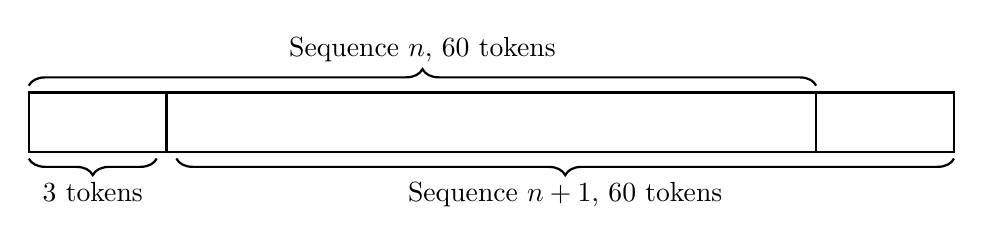
\begin{tikzpicture}[scale=0.25]

                \draw[thick] (0, 0) rectangle (40, 3);
                \draw[thick] (7, 0) rectangle (47, 3);
                \draw [decorate,
                       thick,
                       decoration={brace, amplitude=6pt, mirror},
                       xshift=0pt,
                       yshift=-10pt]
                    (0, 0) -- node[midway, below, yshift=-5] {3 tokens} (6.5, 0);
                \draw [decorate,
                       thick,
                       decoration={brace, amplitude=6pt},
                       xshift=0pt,
                       yshift=10pt]
                    (0, 3) -- node[midway, above, yshift=5] {Sequence $n$, 60 tokens} (40, 3);
                \draw [decorate,
                       thick,
                       decoration={brace, amplitude=6pt, mirror},
                       xshift=0pt,
                       yshift=-10pt]
                 (7.5, 0) -- node[midway, below, yshift=-5] {Sequence $n + 1$, 60 tokens} (47, 0);
            \end{tikzpicture}
            \caption{Chunking the corpus into overlapping sequences}\label{fig:sequences}
        \end{figure}

        There are two options for tokenizing the corpus. The author chose to tokenize by character rather than by word. This means that the vectorized sequences are sequences of characters, and the model is predicting the very next character of each sequence.

        \newpage
        % I have a new hatred for floating wrapped figures. Welcome to a new kind of hell.
        \begin{wrapfigure}[50]{r}[20pt]{0pt}
            \centering
            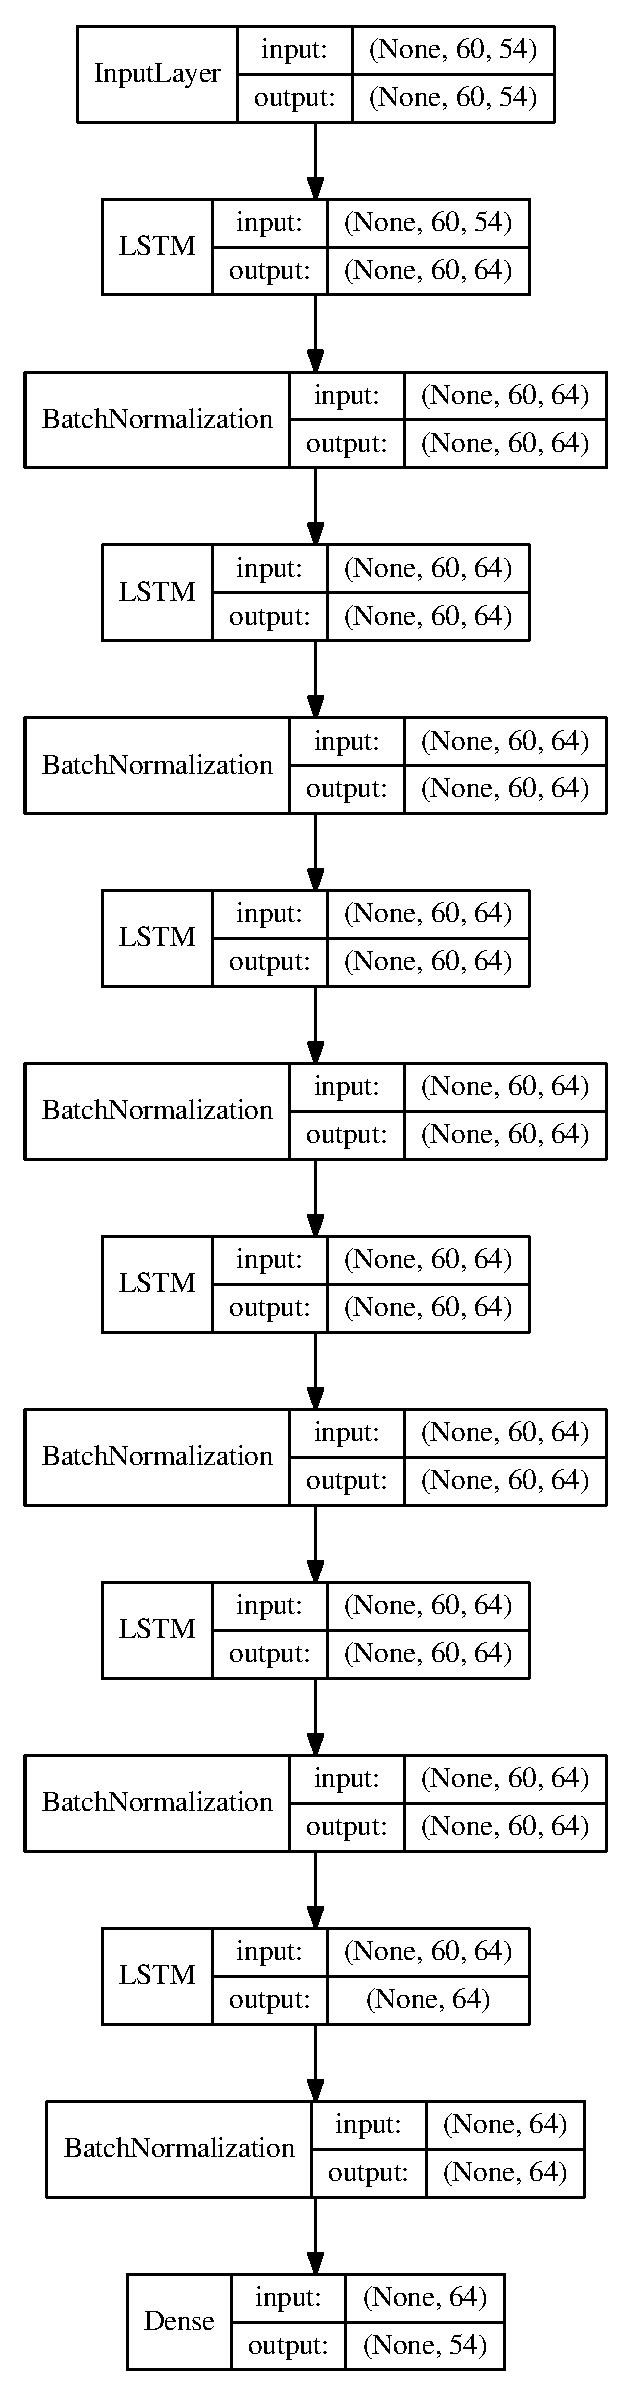
\includegraphics[width=0.39\textwidth]{figures/64x6.eps}
            \caption{A deep and narrow LSTM model using batch normalization}\label{fig:archetecture-64x6}
        \end{wrapfigure}

        Additionally, the sequences overlap a great deal, and contain an enormous amount of redundant data. The dataset in JSON form takes a mere 9.3 megabytes, but in vectorized form takes almost 5 gigabytes. Also note that even though there are only $\sim 37$ thousand tweets by President Trump, the vectorized dataset turns into $\sim 1.1$ \textit{million} sequences.

        Also note that the author trained the experimental models on \textit{all} of President Trump's tweets from his account creation in 2009 to 2018.\todo{Move this to discussion}{}

    \subsection{Model Architectures}
        The author attempted 21 different variations of LSTM models in both height and depth. Most examples and online recommendations were to use relatively shallow networks with height determined by circumstance.\todo{Citation needed?}{}

        One such configuration that showed promise is shown in~\autoref{fig:archetecture-64x6}. This model was composed of six 64-unit LSTM layers with batch normalization. Each configuration used 60 character long sequences as the model input, and a one-hot encoded vector output to indicate the most likely next character in the sequence.

        While the author experimented with regularization, overfitting was not an issue due to the sheer size of the training set. Thus, most of the best performing models used batch normalization rather than some form of dropout.

        Note that the author was not able to significantly outperform his first attempt, which consisted of a single 256-unit LSTM layer without batch normalization or dropout.

    \subsection{Training Variations}
        The author initially used the Root Mean Square Propagation (RMSProp) optimization algorithm on recommendation, but also experimented with Stochastic Gradient Decent (SGD) optimizer. RMSProp is an adaptive optimizer that tunes its learning rate as it runs. The author favors RMSProp due to a considerably faster training time in both time elapsed and number of epochs necessary when compared with SGD.

        When using RMSProp, it was typically only necessary to train for around 5 epochs, depending on the model size, while SGD (even with a higher learning rate) took on average 100 epochs to get comparable results.

    \subsection{Generating New Tweets}
        The neural network takes in a sequence of the training set, and predicts the next token in the corpus. To take a trained network and generate new tweets, we first begin with a seed randomly taken from the corpus. The network predicts the next token in the sequence as an array of probabilities, which is then sampled with some diversity because the intent of the model is to generate new creative work not found in the training set.

        The newly generated token is appended to the seed, which is then shifted down one token. The author chose to repeat this process until the generated portion of the text (excluding the seed) is 280 characters long.

        This process is repeated using several different probability sampling diversities for each randomly chosen seed, resulting in a different piece of generated text for each diversity. The higher the diversity, the more creative the model became, but at the cost of becoming less and less intelligible. The lower the diversity, the more intelligible became, but at the cost of simply repeating portions of text appearing in the corpus.

\section{Results}
    \todoinline{
        \begin{itemize}
            \item Hack validation data into training and produce plots?
            \item Give example tweets?
            \item Grammar, spelling, etc.
            \item Accuracy is meaningless because you're trying to create \textit{new} tweets. This is where the sampling with diversities comes in. The higher diversity the more creative the network is, but the more meaningless it becomes.
            \item Produce a largeish amount of generated tweets.
        \end{itemize}
    }
    \subsection{256 Unit, 1 Layer LSTM}

        \begin{figure}[h]
            \centering
            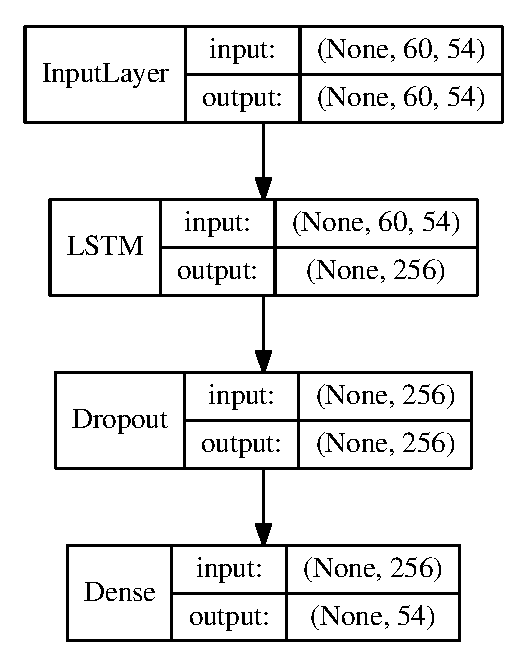
\includegraphics[width=0.4\textwidth]{figures/256dropout.eps}
            \caption{256 unit LSTM model with dropout}\label{fig:archetecture-256}
        \end{figure}

    \subsection{64 Unit, 6 Layer LSTM}
        The following results are using the model shown in~\autoref{fig:archetecture-64x6}.

    \subsection{1024 Unit, 1 Layer LSTM}
    \begin{figure}[h]
        \centering
        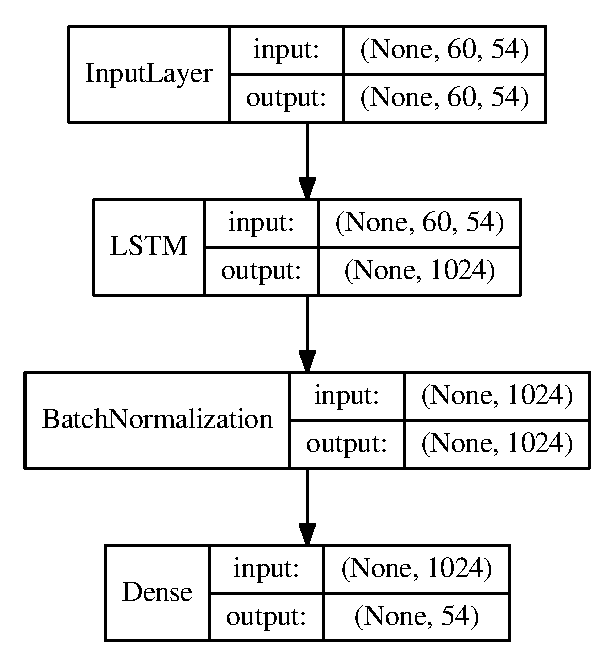
\includegraphics[width=0.5\textwidth]{figures/1024batchnorm.eps}
        \caption{1024 unit LSTM model with batch normalization}\label{fig:archetecture-256}
    \end{figure}

    \subsection{Textgenrnn}
    \begin{figure}[h]
        \centering
        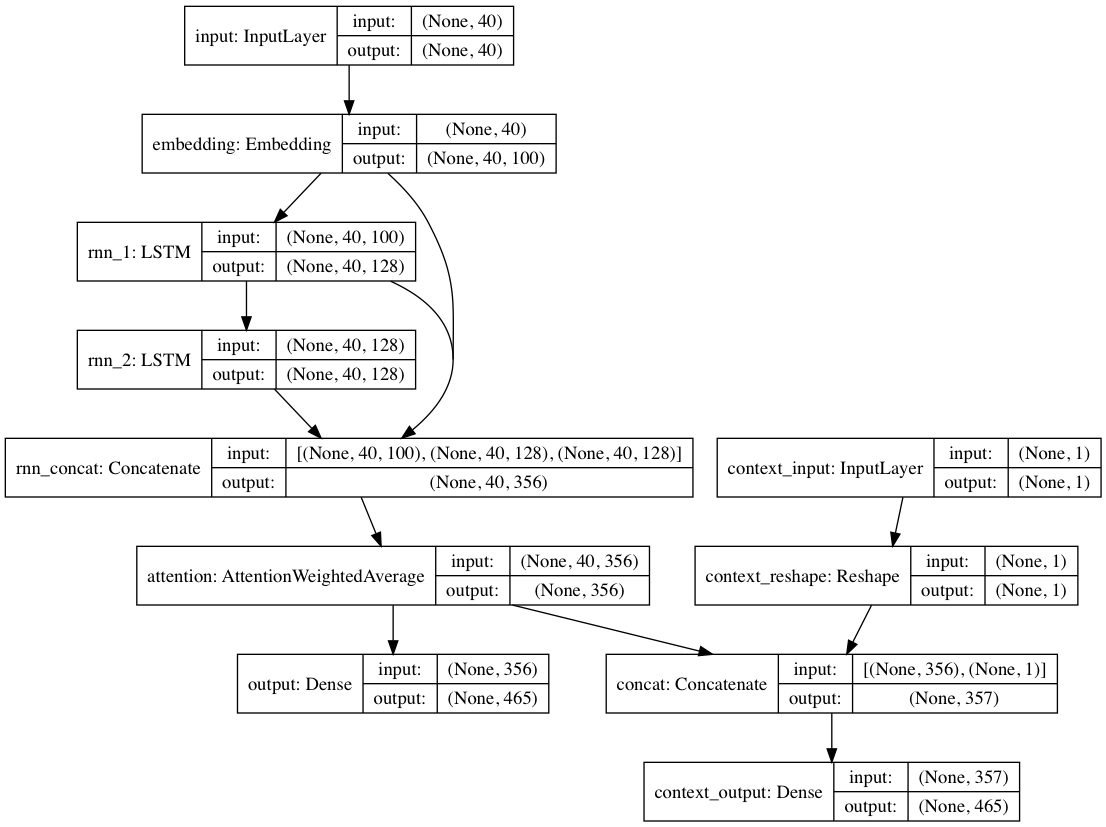
\includegraphics[width=\textwidth]{figures/context_model.png}
        \caption{Textgenrnn architecture}\label{fig:archetecture-256}
    \end{figure}

\section{Discussion}
    \todoinline{
        \begin{itemize}
            \item How good was it?
            \item Accuracy meaningless because attempt is creative generation.
            \item Did it pick up on patterns backed by data?
        \end{itemize}
    }

\section{Future Work}
    \todoinline{
        \begin{itemize}
            \item Word level generation. Instead of each character being mapped to an integer, create a vocab list and map each word to an integer.
            \item Word association norms?
            \item Embeddings?
            \item Combining sources?
            \item Grammar and spelling, part of speech tagging, word association, linguistic features as a component of a GAN
            \item Crowd-sourced adversarial network as a training component?
        \end{itemize}
    }

% Have to use one of the natbib styles. They all suck...
\bibliographystyle{abbrvnat}
% Automatically places a \section*{References}...
\bibliography{paper}
\end{document}
